\chapter{Tuning of weight clipping parameter}
\label{chap:W_CLIP}





In the final part of the previous chapter the procedure of weight clipping was introduced and explained. In this one a systematic approch for weight clipping parameter tuning is developed. The procedure is then tested with several cases, where the difference is in the size of reference sample. It is important to highlight that in this procedure no signal event is given to the network because we are trying to search the optimal $W$ for which the ditribution of $t$ converges after training to a $\chi^2$ ditribution with 96 dofs.

Beside searching the optimal weight clipping for each case, another aim is to find a trend for $W$ in order to avoid a tuning when data samples of new sizes are given to the net. The cases studied for the test are listed below in Table \ref{tab:W_CLIP_TEST_SIZES}.

\begin{table}[H]
	\centering
	\begin{tabular}{c c c c}
		\toprule
		n° of test	&	Reference size	&	Background size	&	Signal size	\\
		\midrule
		1			&	100k			&	20k				&	0			\\
		2			&	200k			&	20k				&	0			\\
		3			&	300k			&	20k				&	0			\\
		4			&	500k			&	20k				&	0			\\
		5			&	1000k			&	20k				&	0			\\
		\bottomrule
	\end{tabular}
	\caption{Sizes of the datasets for different tests.}
	\label{tab:W_CLIP_TEST_SIZES}
\end{table}





\section{A criterion for optimal weight clipping}
As suggested in the previous discussion, the optimal weight clipping is reached when the sampled distribution of $t$ resembles the expected ditribution of a $\chi^2$ with 96 dofs. Therefore, after setting a value for $W$ and sampling a certain number of observed $t$ values, a compatibility test has to be applied with the expected ditribution. A good choice for this purpose is putting the sampled $t$s in a histogram and applying a $\chi^2$ test between the latter and the expected distribution, put in a histogram as well. Now the possible cases are the following:
\begin{itemize}
	\item If the observed $\chi^2$ of the test statistic is beyond an equivalent threshold of $3\sigma$, the observed distribution has converged to the reference one.
	\item If the threshold is not met, the weight clipping has to be lowered or increased depending on the trend of the observed $\chi^2$ of test statistic during training.
	\begin{itemize}
		\item[$\triangleright$] If there is a valley and after reaching a minimum the observed $\chi^2$ begins to grow, the weight clipping has to be lowered.
		\item[$\triangleright$] If there isn't a minimum but the observed $\chi^2$ is still decreasing at the end of training, the weight clipping has to be increased.
	\end{itemize}
\end{itemize}

It is obvious that this method could be computationally very expensive. Finding an optimal value for $W$ requires more trials and every trial requires a certain time as the number of $t$ needed to sample a distribution is $\gtrsim 10^2$. However, a good strategy to save a lot of time can be easily developed.

The starting point of the search should be the case with the smallest size of reference sample. In fact, training the network in this case requires a relative short time (for instance, $\sim 8~\si{h}$), so more trials can be done without an excessive loss of time. Found the optimal $W$ for this case, the next reference sample in increasing order of size should be used for training. The value of optimal $W$ is expected to be greater than the one in the previous case. The reason for this is giving more reference data to the network is equivalent to have more statistic and so the danger of finding divergences in the training is lower. Hence $W$ can be set to a greater value as it is a regularization parameter. Moreover, if the size of reference is slightly increased, it is reasonable thinking that the optimal weight clipping should be slightly greater as well than in the previous case.





\section{Results for optimal weight clipping search}
Only the best results for each case are reported in the Figures below. Results for other trials are reported in Table [INSERIRE LABEL]. In the following figures four plots are given:
\begin{itemize}
	\item The final distribution of the observed $t$ along with the expected distribution at 96 dofs.
	\item A plot of several quantiles of the observed $t$ distribution. The quantiles chosen are 2.5\%, 25\%, 50\%, 75\%, 97.5\%. The most important thing to note in this plot is the plateaux reached during training.
	\item A plot of the observed $\chi^2$ over training related to the test statistic to assert the compatibility of observed $t$ distribution and the expected one.
	\item A plot of the observed $p$-value over training related to the corresponding value of observed $\chi^2$ in the previous plot. It is calculated considering a $\chi^2$ distribution at $N-1$ dofs, where $N$ is the number of bins.
\end{itemize}

\begin{figure}[H]
	\centering
	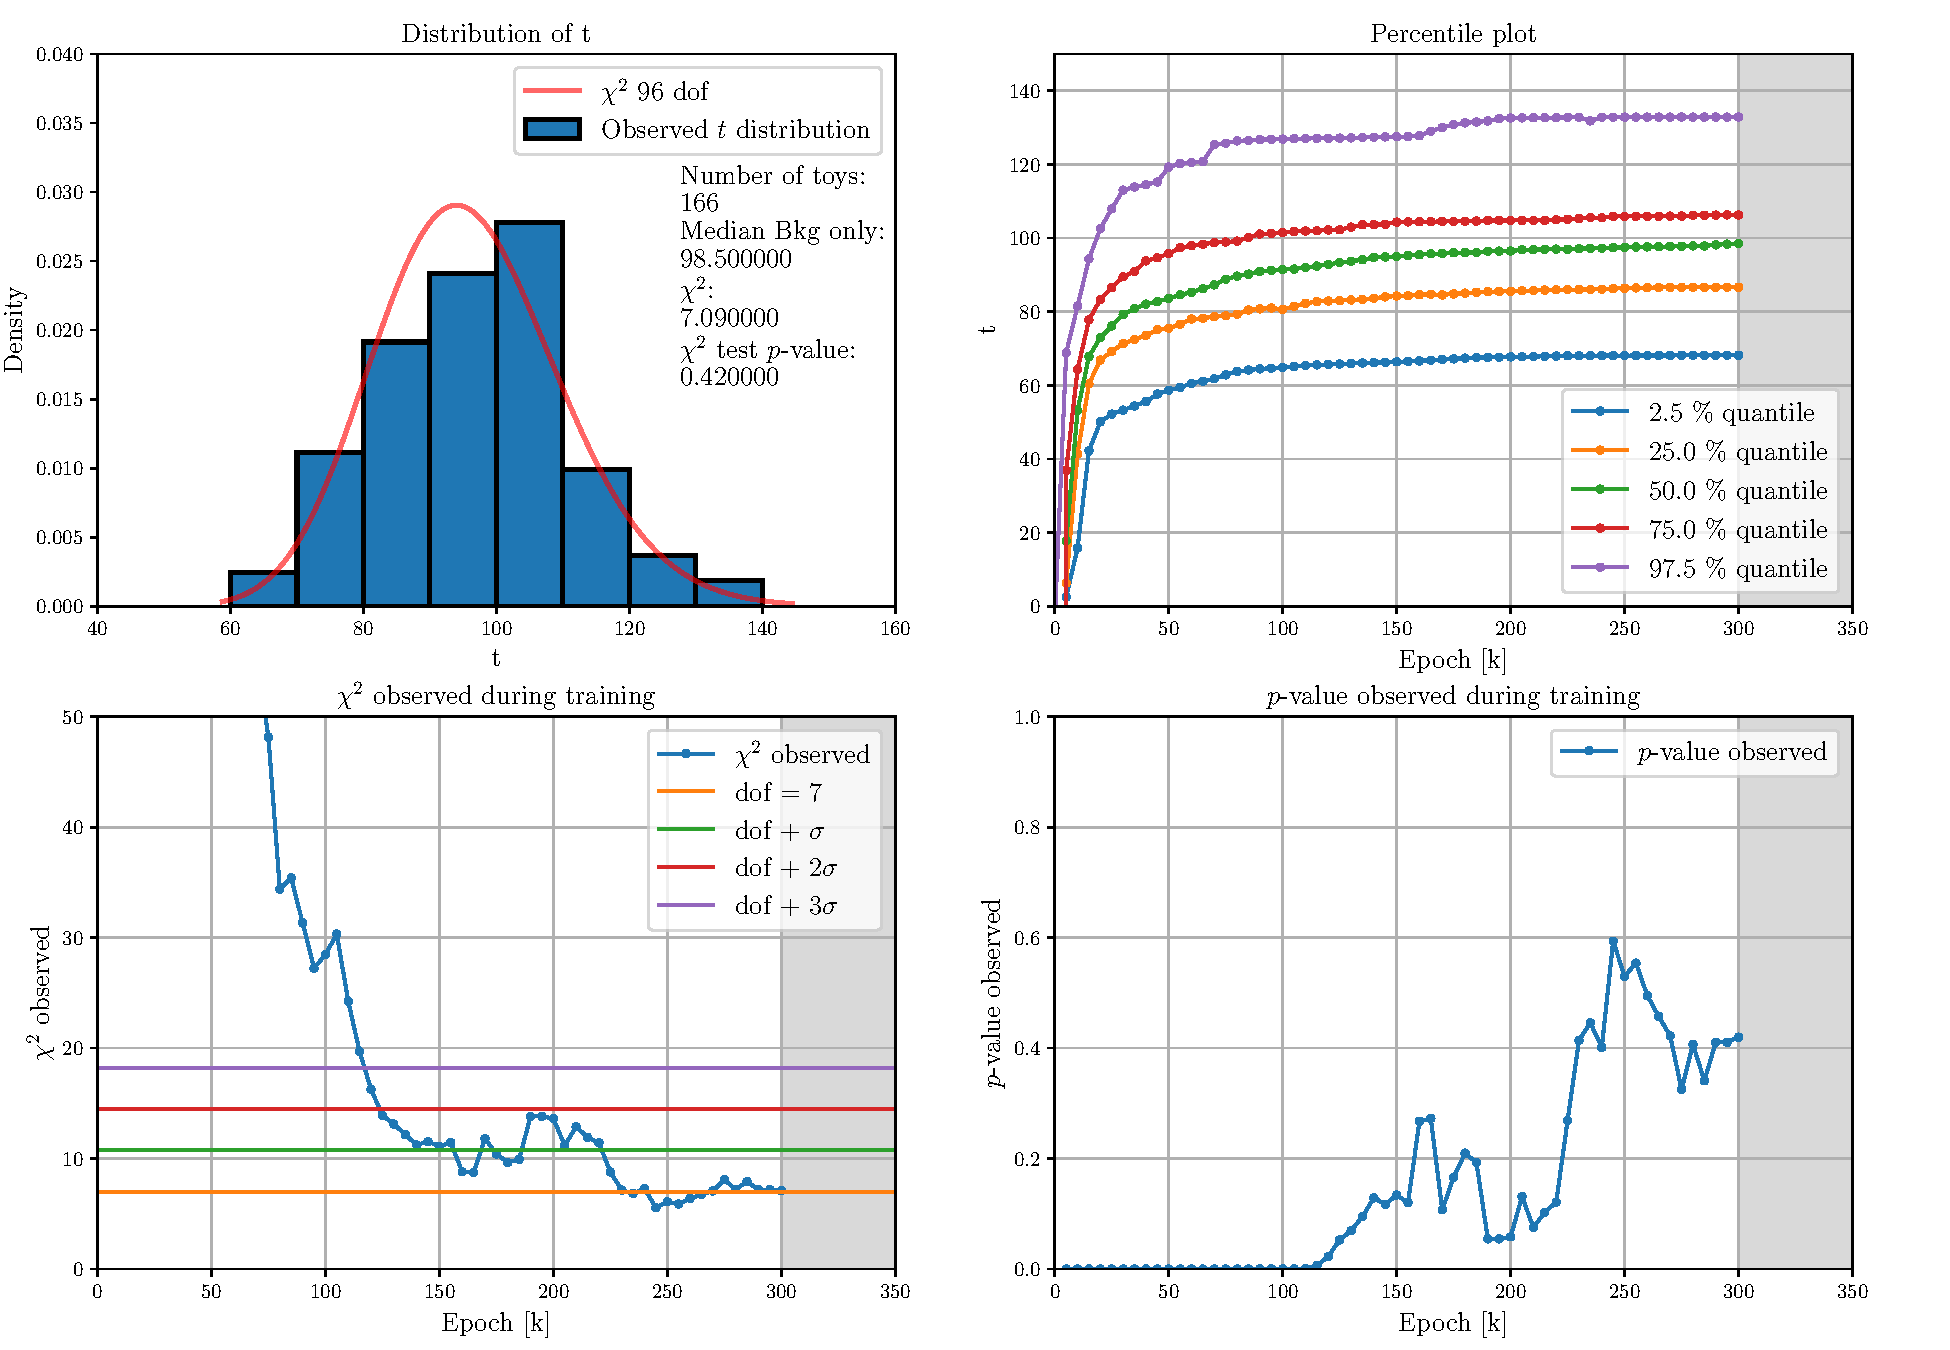
\includegraphics[width=0.9\textwidth]{Python/W_CLIP/ref100000_bkg20000_sig0/data_ref100000_bkg20000_sig0_wclip2-15.pdf}
	\caption{Results of optimal $W$ search for $W=2.15$.}
	\label{fig:REF100000_BKG20000_SIG0_WCLIP2.15}
\end{figure}

\begin{figure}[H]
	\centering
	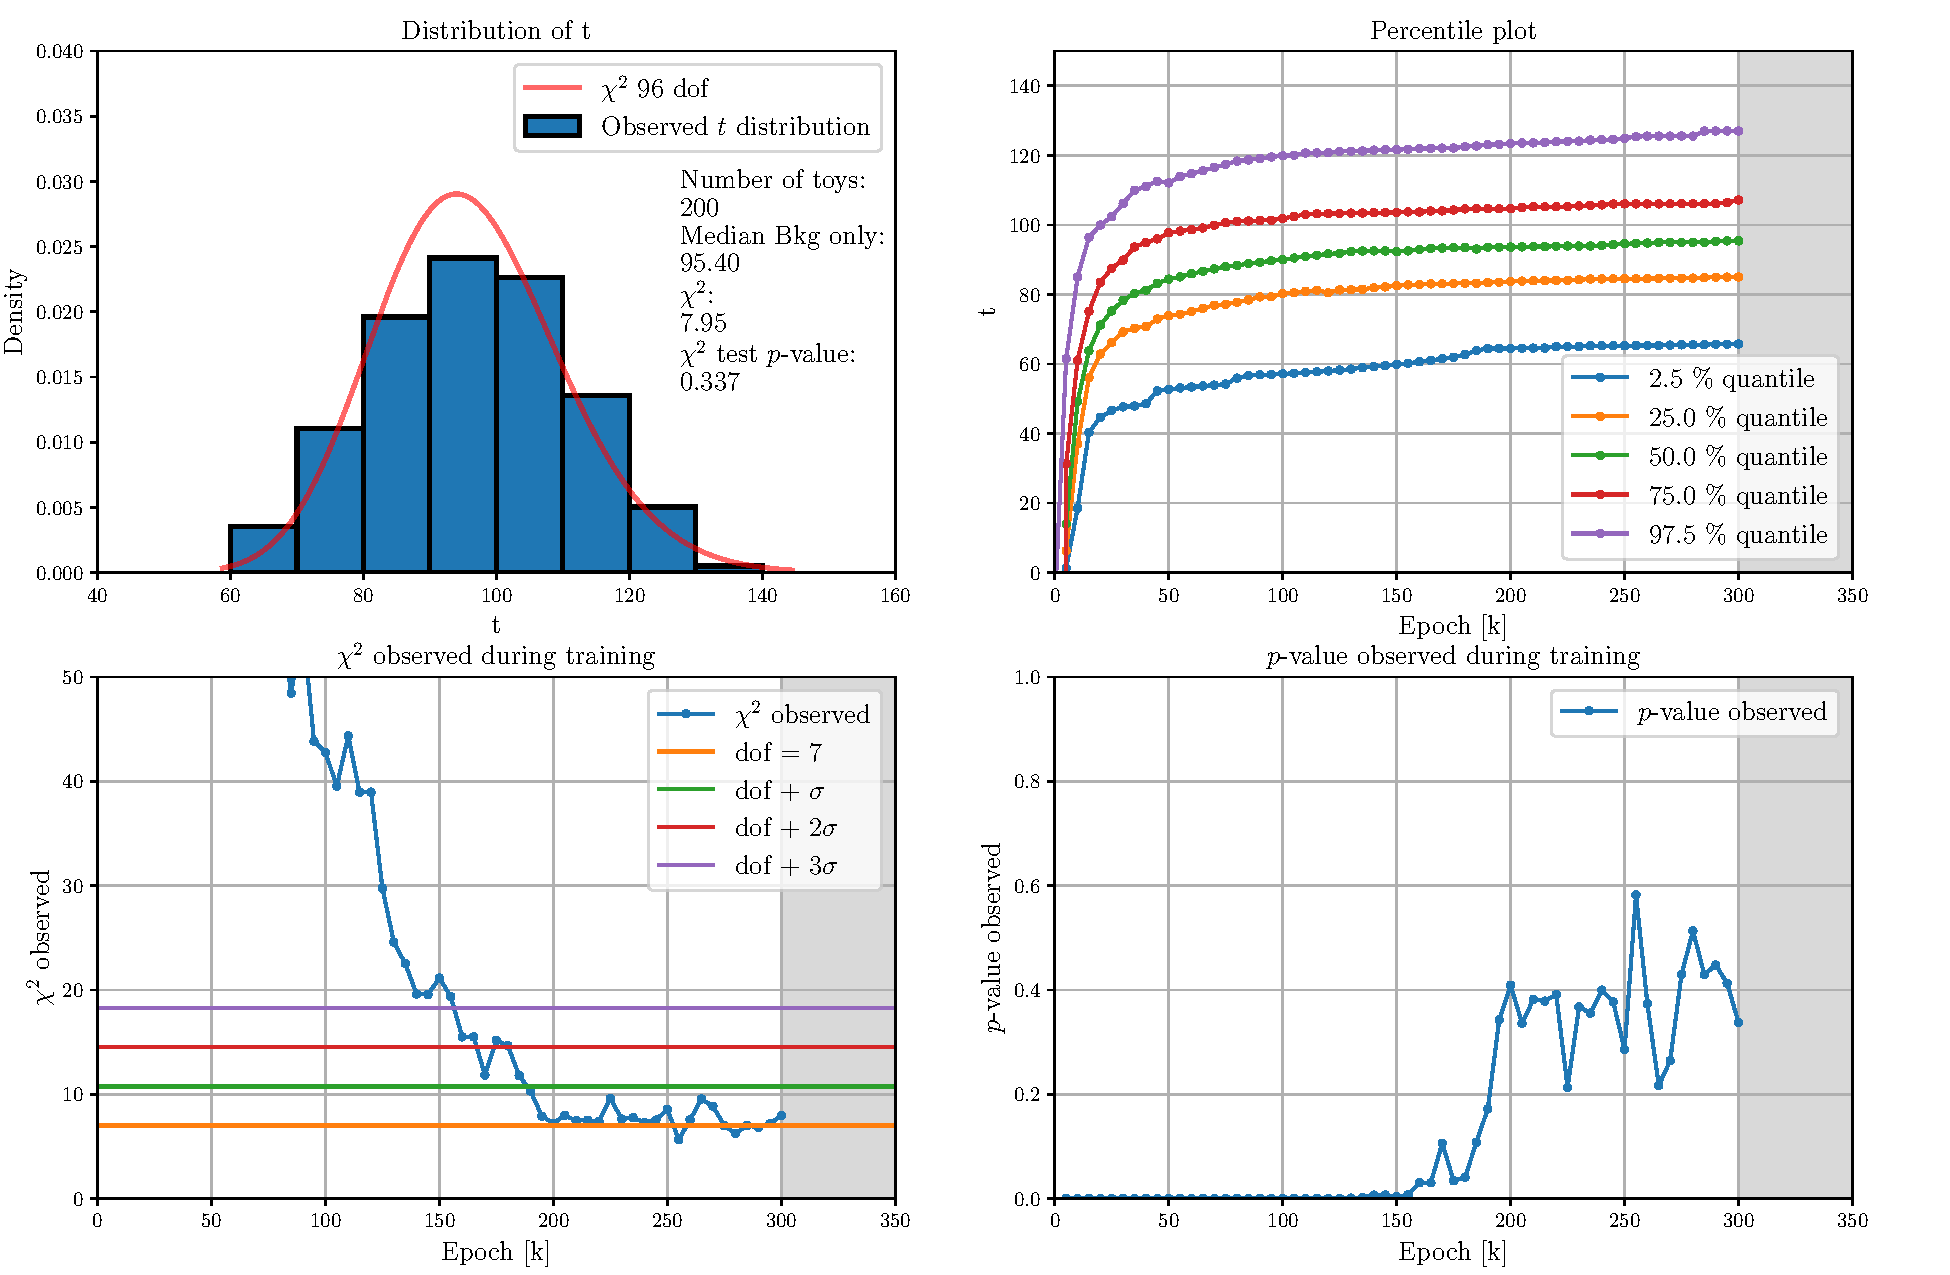
\includegraphics[width=0.9\textwidth]{Python/W_CLIP/ref200000_bkg20000_sig0/data_ref200000_bkg20000_sig0_wclip2-4.pdf}
	\caption{Results of optimal $W$ search for $W=2.4$.}
	\label{fig:REF200000_BKG20000_SIG0_WCLIP2.4}
\end{figure}

\begin{figure}[H]
	\centering
	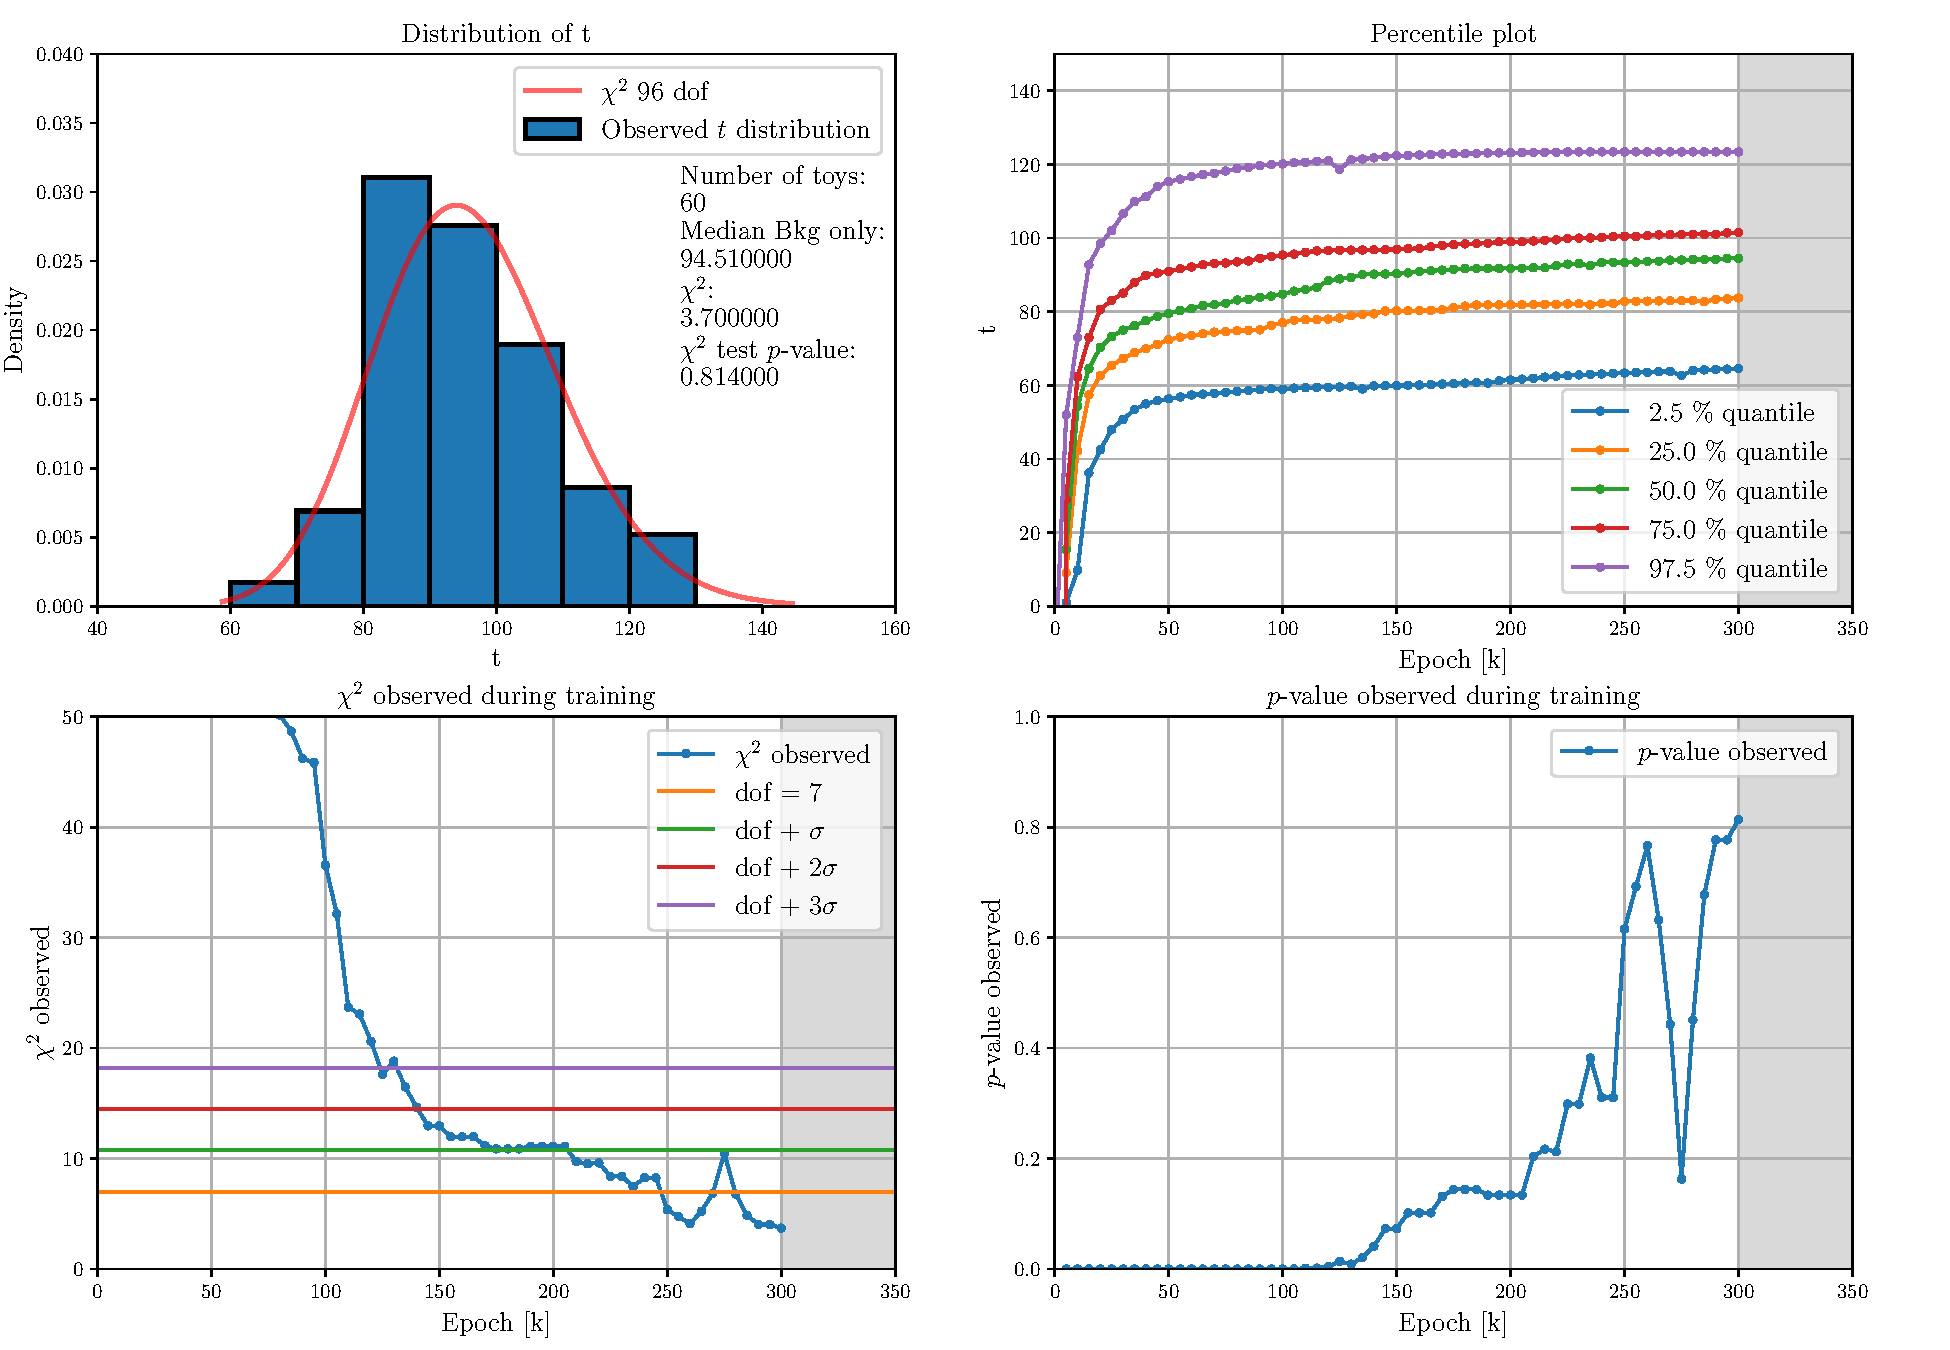
\includegraphics[width=0.9\textwidth]{Python/W_CLIP/ref300000_bkg20000_sig0/data_ref300000_bkg20000_sig0_wclip2-3.pdf}
	\caption{Results of optimal $W$ search for $W=2.3$.}
	\label{fig:REF300000_BKG20000_SIG0_WCLIP2.3}
\end{figure}

\begin{figure}[H]
	\centering
	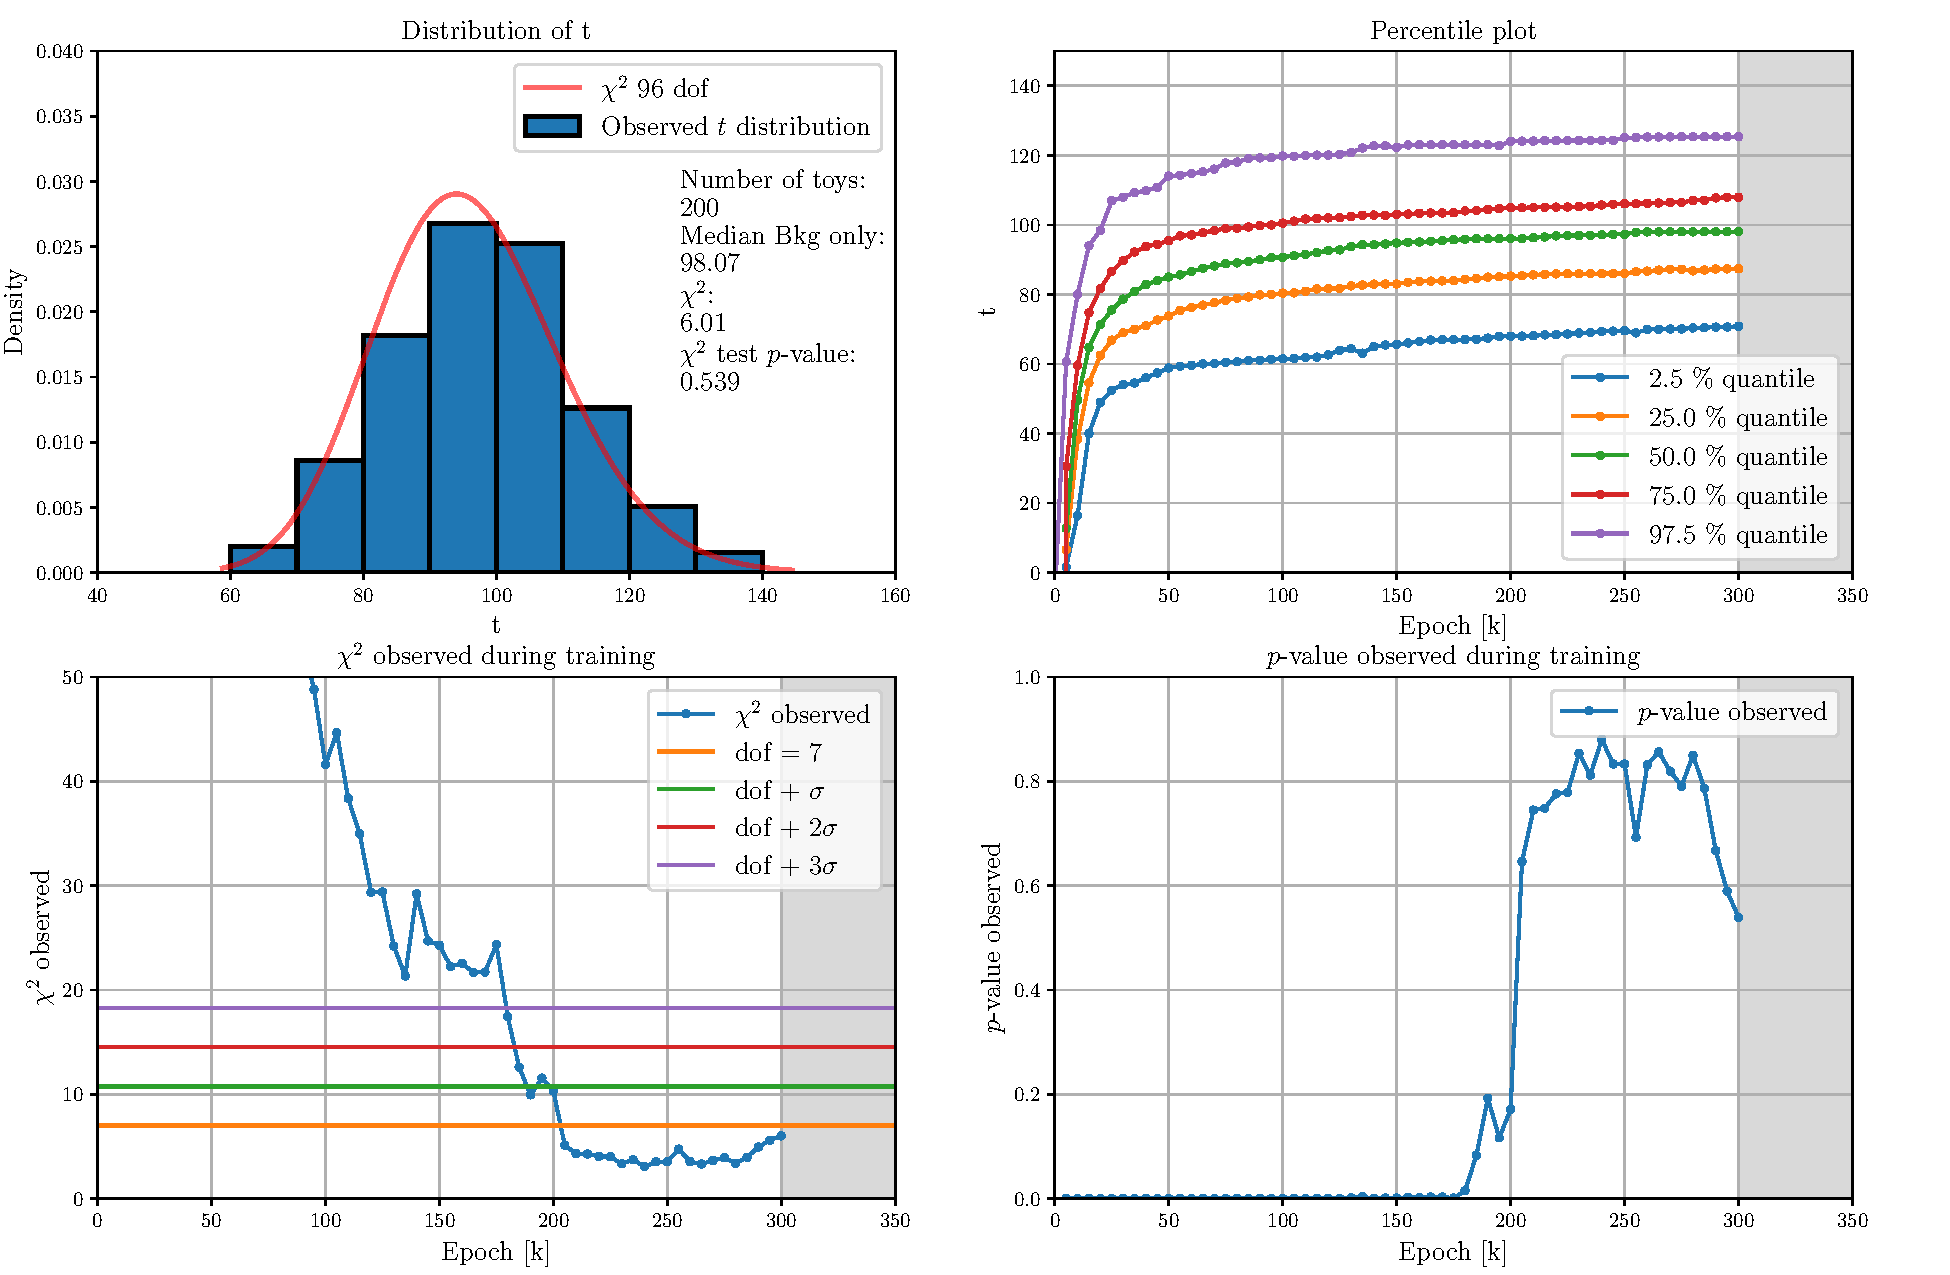
\includegraphics[width=0.9\textwidth]{Python/W_CLIP/ref500000_bkg20000_sig0/data_ref500000_bkg20000_sig0_wclip2-55.pdf}
	\caption{Results of optimal $W$ search for $W=2.55$.}
	\label{fig:REF500000_BKG20000_SIG0_WCLIP2.55}
\end{figure}